\chapter{DF-060 V7 DOGFOOD Release Title Screen And Closeout Six-Pack}\label{record-101}

\noindent{\footnotesize\color{BookMuted}\path{docs/design/DF-060-v7-dogfood-release-title-screen.md}\par}\smallskip

\begin{RecordMeta}
title: DF-060 V7 DOGFOOD release title screen and closeout six-pack
legend: DF
lane: release
priority: medium
keywords:
  - blocklab
  - dogfood
  - release
  - table-surface
  - workflow

\end{RecordMeta}

\section{Framing}\label{record-101-framing}

This cycle pulls the remaining v7 product-truth work into one closeout pass and adds a release-specific DOGFOOD title surface before v7 is considered ready to cut. The title screen should make the release feel intentional, but it must remain a useful terminal documentation entry point rather than a decorative splash screen.

This cycle carries six issues:

\begin{center}
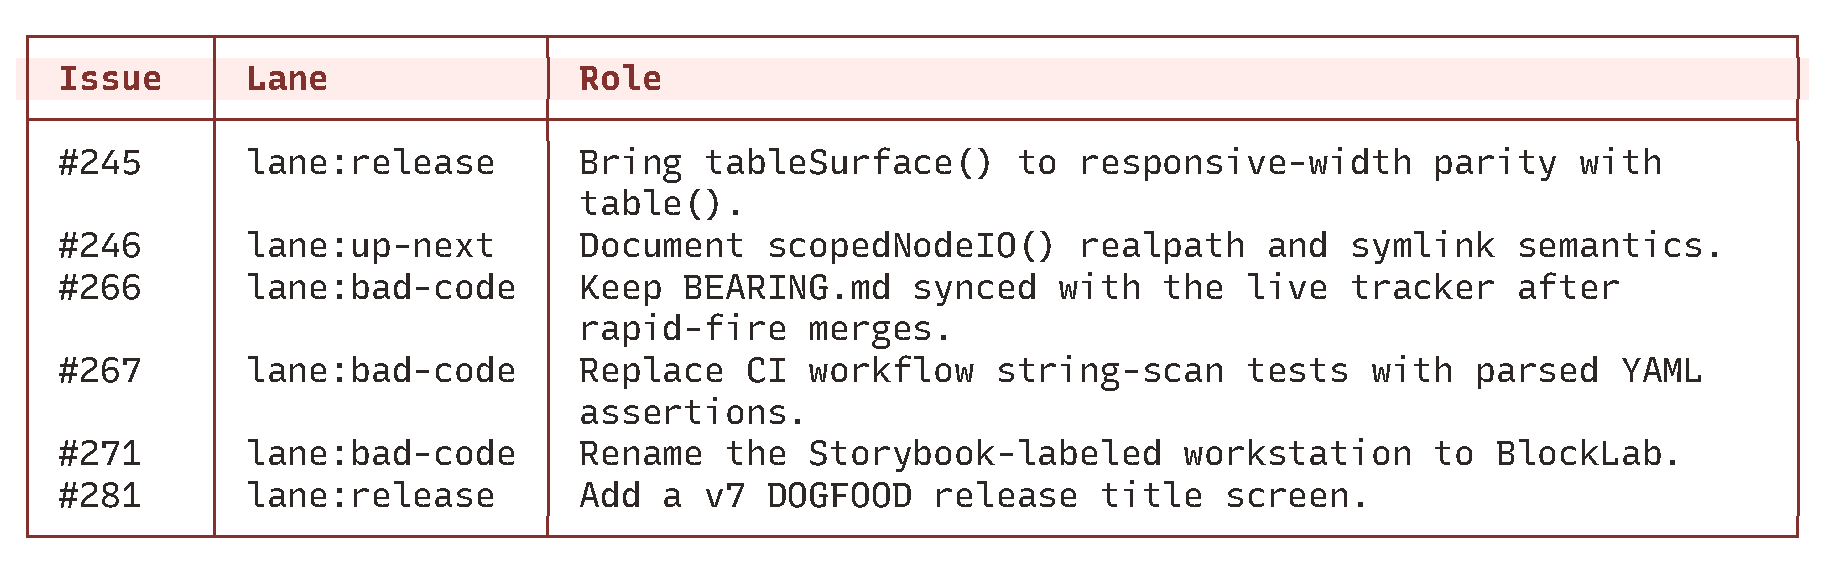
\includegraphics[width=\linewidth]{figures/tables/table-030-g1-1.pdf}
\par\smallskip{\scriptsize\color{BookMuted}Rows 1–6. Actual Bijou table component.}
\end{center}


The design follows a Design Thinking loop:

\begin{itemize}
\tightlist
\item
  observe the remaining release gaps through the live GitHub tracker instead of stale roadmap prose
\item
  frame the work around user-visible release truth and agent-inspectable release proof
\item
  prototype the title screen, BlockLab labels, table parity, lower modes, and workflow guards before treating the cycle as landed
\item
  prove the result with rendered DOGFOOD tests, package/API tests, docs tests, localization gates, and parsed workflow assertions
\end{itemize}

\section{Sponsored Users}\label{record-101-sponsored-users}

\begin{itemize}
\tightlist
\item
  A maintainer preparing v7 needs the issue tracker, roadmap, BEARING, title surface, and release proof to agree without manual reconciliation.
\item
  A TUI builder needs \texttt{t\allowbreak{}a\allowbreak{}b\allowbreak{}l\allowbreak{}e\allowbreak{}S\allowbreak{}u\allowbreak{}r\allowbreak{}f\allowbreak{}a\allowbreak{}c\allowbreak{}e\allowbreak{}(\allowbreak{})} to obey the same width constraints and lower-mode semantics already proven by \texttt{t\allowbreak{}a\allowbreak{}b\allowbreak{}l\allowbreak{}e\allowbreak{}(\allowbreak{})}.
\item
  A component author needs the preview workstation to use a project-owned name, BlockLab, while legacy commands remain available during migration.
\item
  A review agent needs structured workflow assertions, stable release-title facts, and lower-mode output instead of brittle prose or raw string scans.
\end{itemize}

\section{Hills}\label{record-101-hills}

\begin{enumerate}
\def\labelenumi{\arabic{enumi}.}
\tightlist
\item
  A DOGFOOD reader can open the docs app and see a v7 title surface that names the release identity, proof lanes, and navigation options at wide and narrow terminal widths.
\item
  A TUI author can use \texttt{t\allowbreak{}a\allowbreak{}b\allowbreak{}l\allowbreak{}e\allowbreak{}S\allowbreak{}u\allowbreak{}r\allowbreak{}f\allowbreak{}a\allowbreak{}c\allowbreak{}e\allowbreak{}(\allowbreak{})} with explicit width constraints and get output that fits like \texttt{t\allowbreak{}a\allowbreak{}b\allowbreak{}l\allowbreak{}e\allowbreak{}(\allowbreak{})} while preserving row, column, value, and selected-cell facts in lower modes.
\item
  A maintainer can close the v7 issue lane with GitHub, BEARING, ROADMAP, CHANGELOG, workflow tests, BlockLab names, and docs all pointing to the same release truth.
\end{enumerate}

\section{Playback Questions}\label{record-101-playback-questions}

\begin{itemize}
\tightlist
\item
  Does DOGFOOD show release identity without blocking normal documentation navigation?
\item
  Does the title screen lower to static, pipe, and accessible output with release id, release title, proof lane, and navigation facts?
\item
  Does \texttt{t\allowbreak{}a\allowbreak{}b\allowbreak{}l\allowbreak{}e\allowbreak{}S\allowbreak{}u\allowbreak{}r\allowbreak{}f\allowbreak{}a\allowbreak{}c\allowbreak{}e\allowbreak{}(\allowbreak{})} fit constrained widths instead of retaining old intrinsic sizing assumptions?
\item
  Do \texttt{s\allowbreak{}c\allowbreak{}o\allowbreak{}p\allowbreak{}e\allowbreak{}d\allowbreak{}N\allowbreak{}o\allowbreak{}d\allowbreak{}e\allowbreak{}I\allowbreak{}O\allowbreak{}(\allowbreak{})} docs explain realpath-normalized paths and symlink escape rejection with enough precision for callers?
\item
  Can workflow policy tests prove the checkout depth and i18n base behavior by parsing CI YAML instead of searching raw text?
\item
  Do humans see BlockLab, while existing \texttt{s\allowbreak{}t\allowbreak{}o\allowbreak{}r\allowbreak{}y\allowbreak{}b\allowbreak{}o\allowbreak{}o\allowbreak{}k} npm scripts continue to work for one migration window?
\item
  Do BEARING and ROADMAP match the live GitHub tracker after this cycle?
\end{itemize}

\section{Product Shape}\label{record-101-product-shape}

\subsection{DOGFOOD V7 Title, Wide}\label{record-101-dogfood-v7-title-wide}

\begin{CodeBlock}
+ BIJOU DOGFOOD -------------------------------------------+
| V7 Product Truth                                         |
| Blocks prove product surfaces. DOGFOOD proves Blocks.    |
|                                                          |
| Proof lanes: table parity | scoped Node I/O | BlockLab   |
| Release gate: v6 issue-complete, v7 closeout in flight   |
|                                                          |
| [Docs] [Blocks] [BlockLab] [Release Notes]               |
+----------------------------------------------------------+
\end{CodeBlock}

\subsection{DOGFOOD V7 Title, Narrow}\label{record-101-dogfood-v7-title-narrow}

\begin{CodeBlock}
+ BIJOU DOGFOOD ----+
| V7 Product Truth  |
| Blocks prove UX.  |
| lanes: table, io  |
| gate: closeout    |
+-------------------+
\end{CodeBlock}

\subsection{\texorpdfstring{\texttt{t\allowbreak{}a\allowbreak{}b\allowbreak{}l\allowbreak{}e\allowbreak{}S\allowbreak{}u\allowbreak{}r\allowbreak{}f\allowbreak{}a\allowbreak{}c\allowbreak{}e\allowbreak{}(\allowbreak{})} Width Parity}{ Width Parity}}\label{record-101-tablesurface-width-parity}

\begin{CodeBlock}
+ ResponsiveTableSurface -----------------------------+
| Package     Status   Tests                           |
| bijou       ready    1820                            |
| bijou-tui   ready    640                             |
| Layout: fitted to 48 columns                         |
+------------------------------------------------------+
\end{CodeBlock}

\subsection{BlockLab Workbench}\label{record-101-blocklab-workbench}

\begin{CodeBlock}
Bijou BlockLab                         story: notification-system
Stories 12  Families 6  Modes interactive/static/pipe/accessible

+ Preview ------------------------------------------------+
| Notification stack                                      |
| Variant: live                                           |
+---------------------------------------------------------+
\end{CodeBlock}

\section{Lower Modes}\label{record-101-lower-modes}

The title surface should be backed by release metadata so every mode lowers from the same truth.

Static mode:

\begin{CodeBlock}
Bijou DOGFOOD release title. Release V7 Product Truth. Proof lanes: table parity, scoped Node I/O, BlockLab, release title.
\end{CodeBlock}

Pipe mode:

\begin{CodeBlock}
release_id  v7
release_title   V7 Product Truth
proof_lane  table parity
proof_lane  scoped Node I/O
proof_lane  BlockLab
proof_lane  release title
navigation_available    true
\end{CodeBlock}

Accessible mode:

\begin{CodeBlock}
DOGFOOD title screen for V7 Product Truth. Current release proof lanes are table parity, scoped Node I/O, BlockLab, and release title. Navigation remains available after the title.
\end{CodeBlock}

\texttt{t\allowbreak{}a\allowbreak{}b\allowbreak{}l\allowbreak{}e\allowbreak{}S\allowbreak{}u\allowbreak{}r\allowbreak{}f\allowbreak{}a\allowbreak{}c\allowbreak{}e\allowbreak{}(\allowbreak{})} is the surface-native path, so this cycle proves bounded surface width rather than adding a new lowering contract. Semantic table facts remain owned by \texttt{t\allowbreak{}a\allowbreak{}b\allowbreak{}l\allowbreak{}e\allowbreak{}(\allowbreak{})} and \texttt{n\allowbreak{}a\allowbreak{}v\allowbreak{}i\allowbreak{}g\allowbreak{}a\allowbreak{}b\allowbreak{}l\allowbreak{}e\allowbreak{}T\allowbreak{}a\allowbreak{}b\allowbreak{}l\allowbreak{}e\allowbreak{}S\allowbreak{}u\allowbreak{}r\allowbreak{}f\allowbreak{}a\allowbreak{}c\allowbreak{}e\allowbreak{}(\allowbreak{})}:

\begin{CodeBlock}
row-id  bijou
column-id   status
cell-value  ready
layout-variant  fitted
selected-cell   bijou/status
\end{CodeBlock}

\section{Runtime And API Contracts}\label{record-101-runtime-and-api-contracts}

\begin{itemize}
\tightlist
\item
  DOGFOOD release title metadata should be a typed local data structure, not scattered strings in the renderer.
\item
  DOGFOOD visible title strings must go through the DOGFOOD localization catalog.
\item
  \texttt{t\allowbreak{}a\allowbreak{}b\allowbreak{}l\allowbreak{}e\allowbreak{}S\allowbreak{}u\allowbreak{}r\allowbreak{}f\allowbreak{}a\allowbreak{}c\allowbreak{}e\allowbreak{}(\allowbreak{})} should share, reuse, or faithfully mirror the fitted table model already used by \texttt{t\allowbreak{}a\allowbreak{}b\allowbreak{}l\allowbreak{}e\allowbreak{}(\allowbreak{})} instead of growing a second width algorithm.
\item
  \texttt{s\allowbreak{}c\allowbreak{}o\allowbreak{}p\allowbreak{}e\allowbreak{}d\allowbreak{}N\allowbreak{}o\allowbreak{}d\allowbreak{}e\allowbreak{}I\allowbreak{}O\allowbreak{}(\allowbreak{})} docs must state that returned paths can be realpath normalized and that symlink escapes are rejected even when lexical prefixes appear valid.
\item
  Workflow tests should parse \texttt{.\allowbreak{}g\allowbreak{}i\allowbreak{}t\allowbreak{}h\allowbreak{}u\allowbreak{}b\allowbreak{}/\allowbreak{}w\allowbreak{}o\allowbreak{}r\allowbreak{}k\allowbreak{}f\allowbreak{}l\allowbreak{}o\allowbreak{}w\allowbreak{}s\allowbreak{}/\allowbreak{}c\allowbreak{}i\allowbreak{}.\allowbreak{}y\allowbreak{}m\allowbreak{}l} as YAML and inspect \texttt{j\allowbreak{}o\allowbreak{}b\allowbreak{}s\allowbreak{}.\allowbreak{}t\allowbreak{}e\allowbreak{}s\allowbreak{}t\allowbreak{}.\allowbreak{}s\allowbreak{}t\allowbreak{}e\allowbreak{}p\allowbreak{}s} structurally.
\item
  BlockLab should become the canonical human-facing name and \texttt{b\allowbreak{}l\allowbreak{}o\allowbreak{}c\allowbreak{}k\allowbreak{}l\allowbreak{}a\allowbreak{}b\allowbreak{}.\allowbreak{}*} the canonical agent-facing token family, while old \texttt{s\allowbreak{}t\allowbreak{}o\allowbreak{}r\allowbreak{}y\allowbreak{}b\allowbreak{}o\allowbreak{}o\allowbreak{}k} scripts remain as compatibility aliases during this migration window.
\end{itemize}

\section{Accessibility, Localization, And Inspectability}\label{record-101-accessibility-localization-and-inspectability}

\begin{itemize}
\tightlist
\item
  The title screen must expose release title and proof lanes as text, not only border art or color.
\item
  New DOGFOOD strings require \texttt{e\allowbreak{}n}, \texttt{f\allowbreak{}r}, \texttt{e\allowbreak{}s}, and \texttt{d\allowbreak{}e} catalog values.
\item
  \texttt{n\allowbreak{}p\allowbreak{}m\allowbreak{} \allowbreak{}r\allowbreak{}u\allowbreak{}n\allowbreak{} \allowbreak{}d\allowbreak{}o\allowbreak{}g\allowbreak{}f\allowbreak{}o\allowbreak{}o\allowbreak{}d\allowbreak{}:\allowbreak{}i\allowbreak{}1\allowbreak{}8\allowbreak{}n\allowbreak{}:\allowbreak{}c\allowbreak{}o\allowbreak{}m\allowbreak{}p\allowbreak{}l\allowbreak{}e\allowbreak{}t\allowbreak{}e} and \texttt{n\allowbreak{}p\allowbreak{}m\allowbreak{} \allowbreak{}r\allowbreak{}u\allowbreak{}n\allowbreak{} \allowbreak{}d\allowbreak{}o\allowbreak{}g\allowbreak{}f\allowbreak{}o\allowbreak{}o\allowbreak{}d\allowbreak{}:\allowbreak{}i\allowbreak{}1\allowbreak{}8\allowbreak{}n\allowbreak{}:\allowbreak{}c\allowbreak{}h\allowbreak{}e\allowbreak{}c\allowbreak{}k} are part of the merge gate.
\item
  Agent-facing facts should include release id, release title, proof lane ids, navigation availability, table row ids, table column ids, and selected cell identity.
\item
  No title-screen behavior should depend on wall-clock time, network state, or live GitHub API data.
\end{itemize}

\section{Implementation Slices}\label{record-101-implementation-slices}

\begin{enumerate}
\def\labelenumi{\arabic{enumi}.}
\tightlist
\item
  Shape the cycle: create issue \#281, write this design doc, push the branch, and open the early PR.
\item
  Write RED tests for release-title rendering/lower modes, tableSurface width parity, scopedNodeIO docs, parsed workflow assertions, BlockLab labels, and tracker sync.
\item
  Implement \texttt{t\allowbreak{}a\allowbreak{}b\allowbreak{}l\allowbreak{}e\allowbreak{}S\allowbreak{}u\allowbreak{}r\allowbreak{}f\allowbreak{}a\allowbreak{}c\allowbreak{}e\allowbreak{}(\allowbreak{})} width parity and lower-mode facts.
\item
  Document \texttt{s\allowbreak{}c\allowbreak{}o\allowbreak{}p\allowbreak{}e\allowbreak{}d\allowbreak{}N\allowbreak{}o\allowbreak{}d\allowbreak{}e\allowbreak{}I\allowbreak{}O\allowbreak{}(\allowbreak{})} realpath and symlink semantics.
\item
  Rename visible Storybook workstation language to BlockLab while keeping compatibility script aliases.
\item
  Add the v7 DOGFOOD release title metadata, route/guide integration, localization strings, and lower-mode proof.
\item
  Sync BEARING, ROADMAP, CHANGELOG, and issue metadata with GitHub.
\item
  Run focused tests, DOGFOOD i18n gates, docs inventory, lint, typecheck, full test suite, self-review, and PR readiness.
\end{enumerate}

\section{Tests To Write First}\label{record-101-tests-to-write-first}

\begin{itemize}
\tightlist
\item
  \texttt{t\allowbreak{}e\allowbreak{}s\allowbreak{}t\allowbreak{}s\allowbreak{}/\allowbreak{}c\allowbreak{}y\allowbreak{}c\allowbreak{}l\allowbreak{}e\allowbreak{}s\allowbreak{}/\allowbreak{}D\allowbreak{}F\allowbreak{}-\allowbreak{}0\allowbreak{}6\allowbreak{}0\allowbreak{}/\allowbreak{}v\allowbreak{}7\allowbreak{}-\allowbreak{}d\allowbreak{}o\allowbreak{}g\allowbreak{}f\allowbreak{}o\allowbreak{}o\allowbreak{}d\allowbreak{}-\allowbreak{}r\allowbreak{}e\allowbreak{}l\allowbreak{}e\allowbreak{}a\allowbreak{}s\allowbreak{}e\allowbreak{}-\allowbreak{}t\allowbreak{}i\allowbreak{}t\allowbreak{}l\allowbreak{}e\allowbreak{}-\allowbreak{}s\allowbreak{}c\allowbreak{}r\allowbreak{}e\allowbreak{}e\allowbreak{}n\allowbreak{}.\allowbreak{}t\allowbreak{}e\allowbreak{}s\allowbreak{}t\allowbreak{}.\allowbreak{}t\allowbreak{}s}
\item
  \texttt{t\allowbreak{}e\allowbreak{}s\allowbreak{}t\allowbreak{}s\allowbreak{}/\allowbreak{}c\allowbreak{}y\allowbreak{}c\allowbreak{}l\allowbreak{}e\allowbreak{}s\allowbreak{}/\allowbreak{}D\allowbreak{}X\allowbreak{}-\allowbreak{}0\allowbreak{}3\allowbreak{}7\allowbreak{}/\allowbreak{}t\allowbreak{}a\allowbreak{}b\allowbreak{}l\allowbreak{}e\allowbreak{}-\allowbreak{}s\allowbreak{}u\allowbreak{}r\allowbreak{}f\allowbreak{}a\allowbreak{}c\allowbreak{}e\allowbreak{}-\allowbreak{}w\allowbreak{}i\allowbreak{}d\allowbreak{}t\allowbreak{}h\allowbreak{}-\allowbreak{}p\allowbreak{}a\allowbreak{}r\allowbreak{}i\allowbreak{}t\allowbreak{}y\allowbreak{}.\allowbreak{}t\allowbreak{}e\allowbreak{}s\allowbreak{}t\allowbreak{}.\allowbreak{}t\allowbreak{}s}
\item
  \texttt{t\allowbreak{}e\allowbreak{}s\allowbreak{}t\allowbreak{}s\allowbreak{}/\allowbreak{}c\allowbreak{}y\allowbreak{}c\allowbreak{}l\allowbreak{}e\allowbreak{}s\allowbreak{}/\allowbreak{}D\allowbreak{}X\allowbreak{}-\allowbreak{}0\allowbreak{}2\allowbreak{}9\allowbreak{}/\allowbreak{}s\allowbreak{}c\allowbreak{}o\allowbreak{}p\allowbreak{}e\allowbreak{}d\allowbreak{}-\allowbreak{}n\allowbreak{}o\allowbreak{}d\allowbreak{}e\allowbreak{}-\allowbreak{}i\allowbreak{}o\allowbreak{}-\allowbreak{}d\allowbreak{}o\allowbreak{}c\allowbreak{}s\allowbreak{}.\allowbreak{}t\allowbreak{}e\allowbreak{}s\allowbreak{}t\allowbreak{}.\allowbreak{}t\allowbreak{}s}
\item
  \texttt{t\allowbreak{}e\allowbreak{}s\allowbreak{}t\allowbreak{}s\allowbreak{}/\allowbreak{}c\allowbreak{}y\allowbreak{}c\allowbreak{}l\allowbreak{}e\allowbreak{}s\allowbreak{}/\allowbreak{}W\allowbreak{}F\allowbreak{}-\allowbreak{}1\allowbreak{}2\allowbreak{}6\allowbreak{}/\allowbreak{}v\allowbreak{}7\allowbreak{}-\allowbreak{}c\allowbreak{}l\allowbreak{}o\allowbreak{}s\allowbreak{}e\allowbreak{}o\allowbreak{}u\allowbreak{}t\allowbreak{}-\allowbreak{}t\allowbreak{}r\allowbreak{}a\allowbreak{}c\allowbreak{}k\allowbreak{}e\allowbreak{}r\allowbreak{}-\allowbreak{}s\allowbreak{}y\allowbreak{}n\allowbreak{}c\allowbreak{}.\allowbreak{}t\allowbreak{}e\allowbreak{}s\allowbreak{}t\allowbreak{}.\allowbreak{}t\allowbreak{}s}
\item
  \texttt{s\allowbreak{}c\allowbreak{}r\allowbreak{}i\allowbreak{}p\allowbreak{}t\allowbreak{}s\allowbreak{}/\allowbreak{}h\allowbreak{}o\allowbreak{}o\allowbreak{}k\allowbreak{}s\allowbreak{}.\allowbreak{}t\allowbreak{}e\allowbreak{}s\allowbreak{}t\allowbreak{}.\allowbreak{}t\allowbreak{}s} structured CI workflow assertions
\item
  Existing DF-027/DF-069 BlockLab rename tests updated from Storybook labels
\end{itemize}

\section{Acceptance Criteria}\label{record-101-acceptance-criteria}

\begin{itemize}
\tightlist
\item
  PR closes \#245, \#246, \#266, \#267, \#271, and \#281.
\item
  v7 has no open tracker issues after the PR merges, unless new issue triage explicitly says otherwise.
\item
  DOGFOOD has a v7 release title screen with wide, narrow, static, pipe, and accessible proof.
\item
  \texttt{t\allowbreak{}a\allowbreak{}b\allowbreak{}l\allowbreak{}e\allowbreak{}S\allowbreak{}u\allowbreak{}r\allowbreak{}f\allowbreak{}a\allowbreak{}c\allowbreak{}e\allowbreak{}(\allowbreak{})} width behavior is deterministic under constrained terminal widths and preserves semantic facts.
\item
  \texttt{s\allowbreak{}c\allowbreak{}o\allowbreak{}p\allowbreak{}e\allowbreak{}d\allowbreak{}N\allowbreak{}o\allowbreak{}d\allowbreak{}e\allowbreak{}I\allowbreak{}O\allowbreak{}(\allowbreak{})} realpath/symlink semantics are documented in package docs.
\item
  CI workflow guard tests parse YAML and validate the actual test job checkout and i18n base paths.
\item
  BlockLab is the canonical visible name, with compatibility aliases for old \texttt{s\allowbreak{}t\allowbreak{}o\allowbreak{}r\allowbreak{}y\allowbreak{}b\allowbreak{}o\allowbreak{}o\allowbreak{}k} npm scripts.
\item
  All new or changed DOGFOOD localization strings are translated in every supported locale.
\end{itemize}

\section{Risks And Guardrails}\label{record-101-risks-and-guardrails}

\begin{itemize}
\tightlist
\item
  Do not turn the title screen into a blocking splash page. It is a docs entry surface.
\item
  Do not rename legacy \texttt{s\allowbreak{}t\allowbreak{}o\allowbreak{}r\allowbreak{}y\allowbreak{}b\allowbreak{}o\allowbreak{}o\allowbreak{}k} script aliases without a migration window.
\item
  Do not use live GitHub data inside deterministic tests.
\item
  Do not broaden table work into a full table redesign; target \texttt{t\allowbreak{}a\allowbreak{}b\allowbreak{}l\allowbreak{}e\allowbreak{}S\allowbreak{}u\allowbreak{}r\allowbreak{}f\allowbreak{}a\allowbreak{}c\allowbreak{}e\allowbreak{}(\allowbreak{})} parity only.
\item
  Do not make BEARING/ROADMAP the source of truth. They mirror GitHub Issues.
\end{itemize}

